\section{Results}\label{sec:results}
%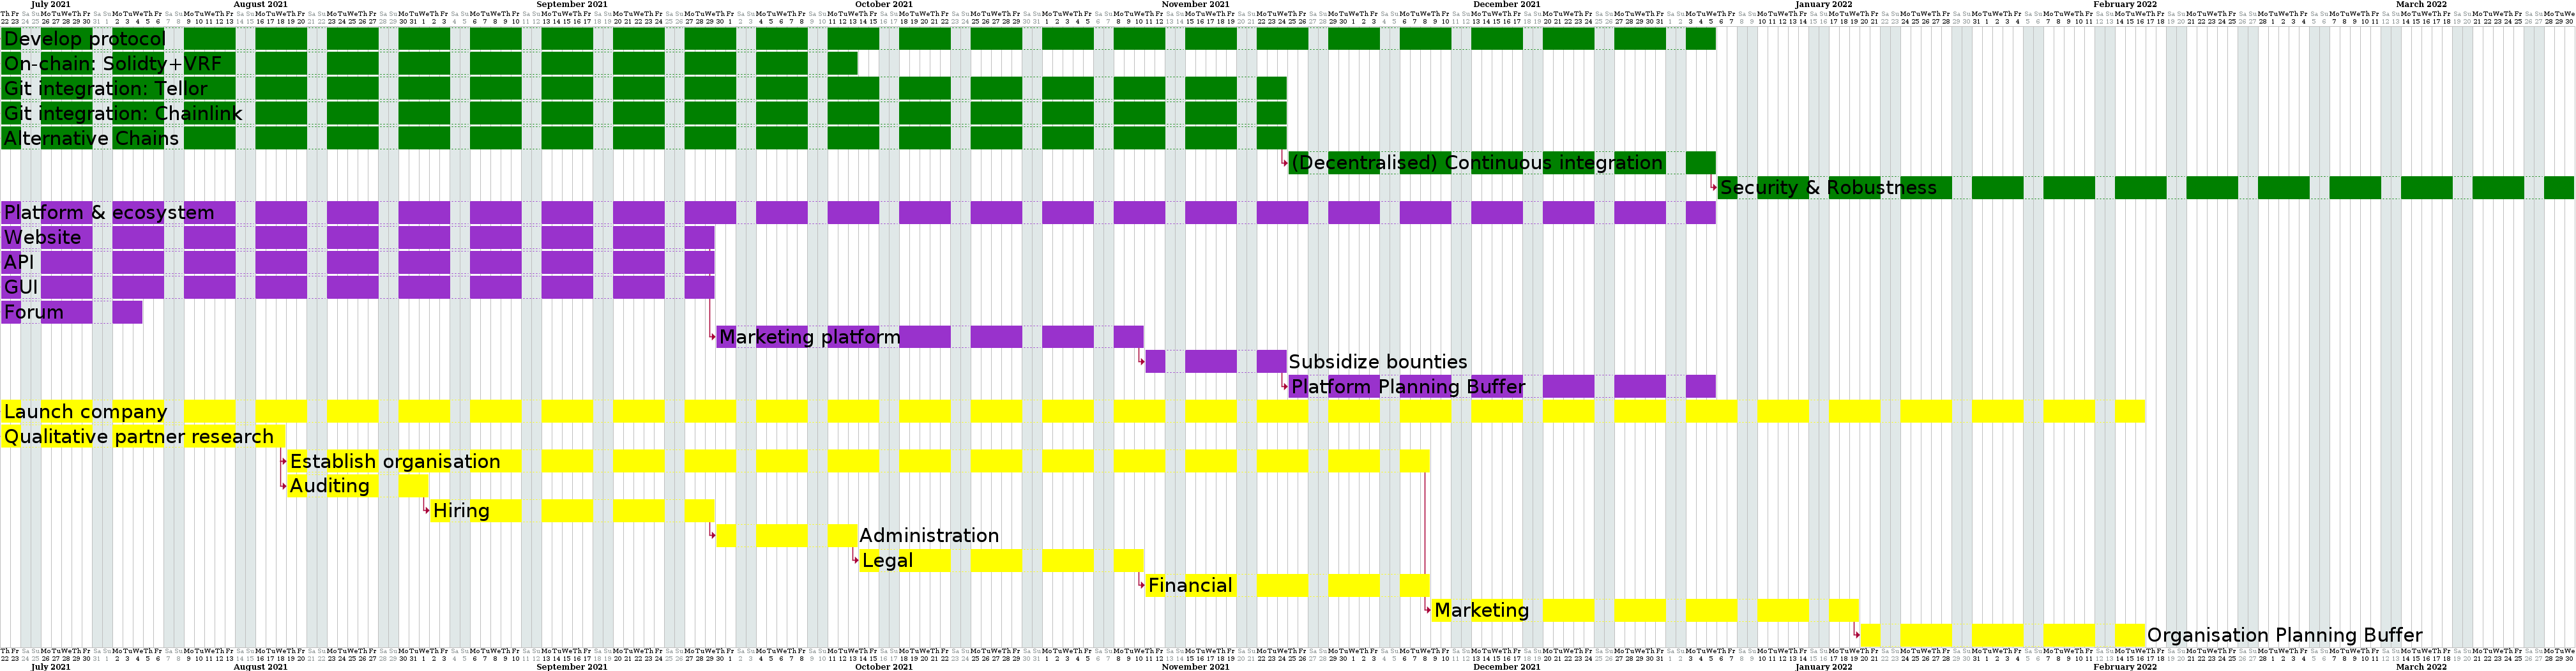
\includepdf{Images/created.png}
\Cref{fig:gantt} contains the Gantt chart that is generated to plan the development of the TruCol company. One can observe that several of the development-activities can be performed in parallel, these are accordingly stacked vertically. Dependencies of outputs of activities imply a "stairway" pattern in the Gantt chart. 
\clearpage
\begin{sidewaysfigure}[ht!]
%\begin{sidewaysfigure}[H]
\hspace*{-0cm}   
    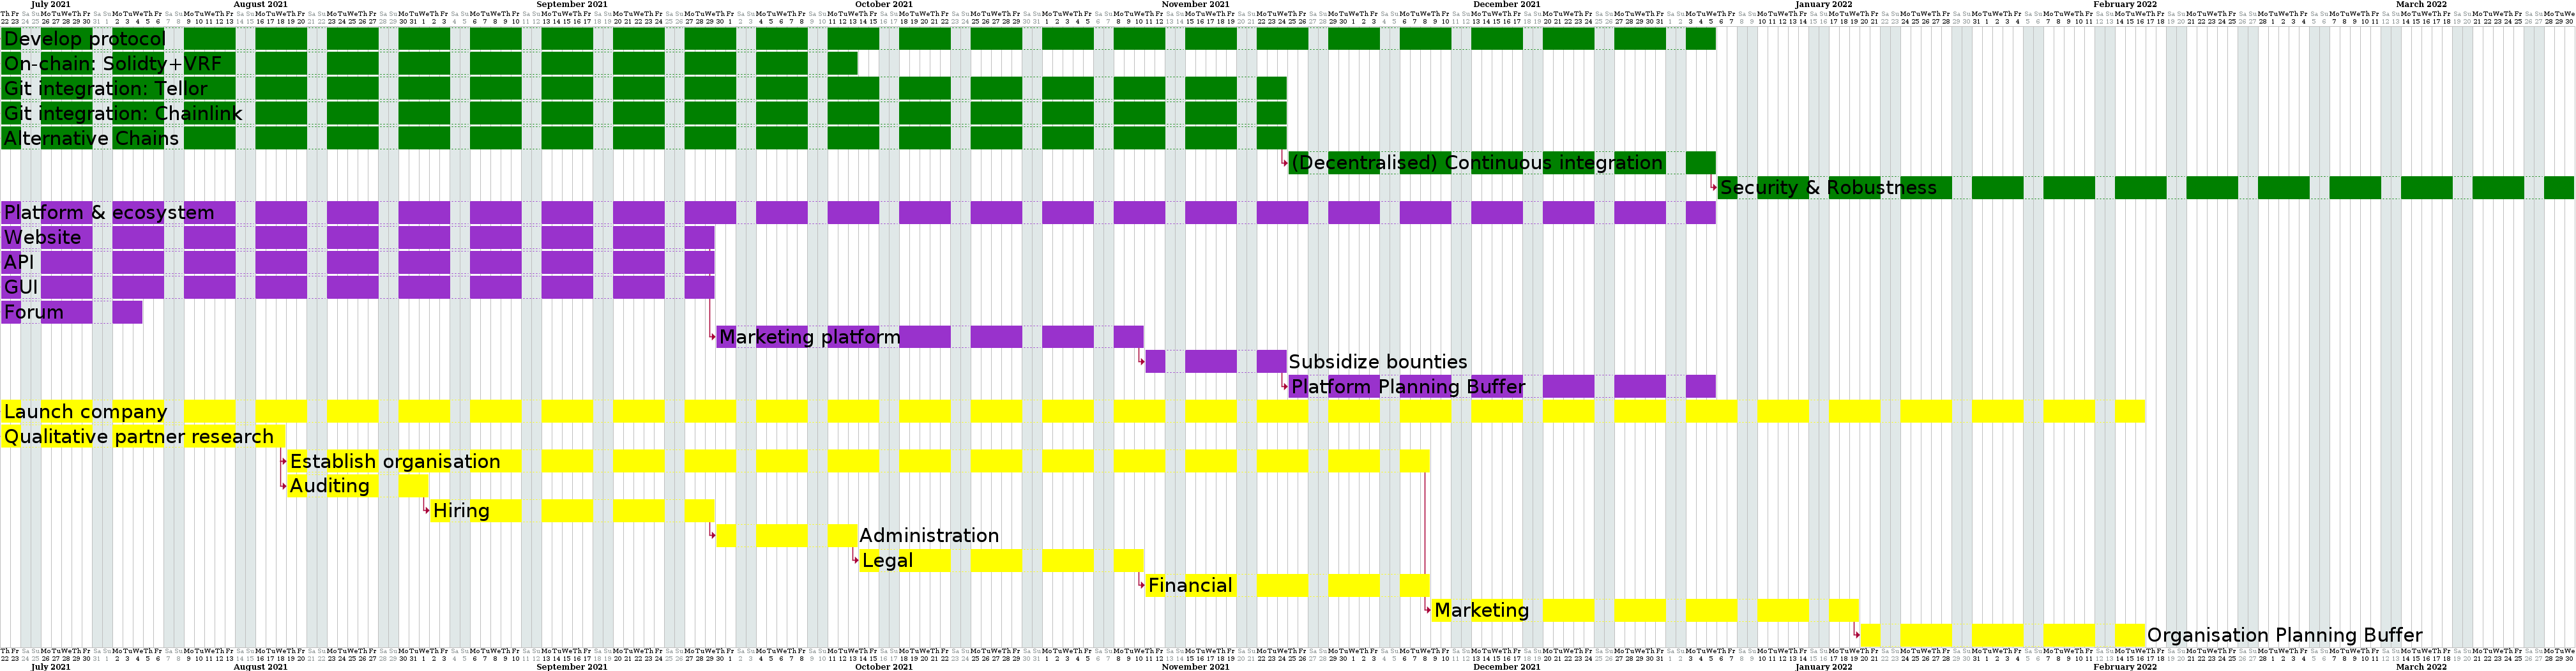
\includegraphics[width=775pt]{Images/created.png}
    \caption{Gantt chart that is generated to plan the development of the TruCol company. (Source code in appendices, and on github.com/trucol/Roadmap).}
    \label{fig:gantt}
\end{sidewaysfigure}
\clearpage
\section{Cost estimates}
After multiplying the amount of labour hours with their respective hourly labour costs, a total estimated labour costs of \euro$470.400,-$ is generated. This is composed of:
\begin{itemize}
	\item Decentralised Tech Developent: \euro$252.000,-$ 
	\item Platform Developent: \euro$112.000,-$ 
	\item Business Development \euro$106.400,-$ 
\end{itemize}
An additional \euro$100.000,-$ are included for bounty subsidation and as a buffer, yielding a total expected cost to create a healthy company of roughly \euro$470.000+$\euro$100.000=$\euro$570.000,-$ which is rounded to approximately .6 Meuro.